\chapter{Cabling, Switching and Network Fabric}

\section{The Physical Medium: Copper and Optical Fiber}
The network is the vascular system of the datacenter. The evolution of traffic density has marked the progressive abandonment of copper in favor of optical fiber.

\subsection{Copper Cables and Ethernet}
Historically, computer networks faced the problem of collisions on shared cables. A widespread topology was the \textbf{Token Ring (IEEE 802.5)}, a physical ring network in which an electronic "token" was passed between computers: only those holding the token could transmit. Although it guaranteed predictable latency, the failure of a single cable or node paralyzed the entire ring. Ethernet won the commercial battle thanks to the star topology and the CSMA/CD protocol, much more robust and flexible but prone to inefficiencies and collisions at high loads before the introduction of switching.

Regarding cabling, data centers relied heavily on copper (e.g. the old \textbf{Cat 5} or Cat 5e cables which limited speeds to 100 Mbps or 1 Gbps). The physical limits of copper (crosstalk and signal attenuation) and the need to manage a precise \textit{pin-out} for contact alignment made evolution increasingly complex. 
Today, the traditional copper cable (Ethernet standard with RJ45 connector) is confined to the practical limit of \textbf{10 Gbps (Cat 6A)}. Going further with standards like Cat 7 or Cat 8 is impractical: the cables become thick, rigid, and difficult to manage (\textit{cable management} is vital, as messy cabling blocks airflow and destroys the thermal efficiency of the rack).

\subsection{Optical Fiber and Transceivers}
\begin{figure}[H]
    \centering
    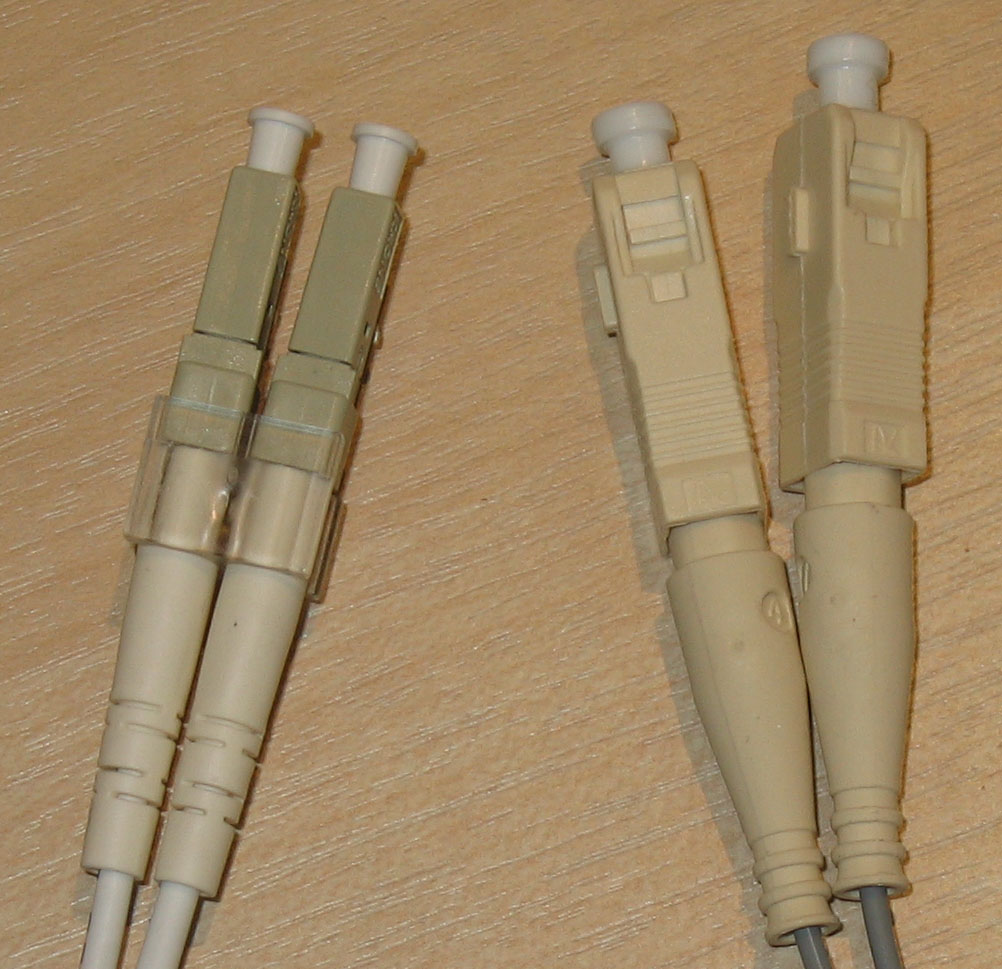
\includegraphics[width=0.6\textwidth]{images/fiber_connectors.jpg}
    \caption{Optical fiber connectors (LC and SC compared).}
\end{figure}
Optical transmission eliminates thermal dissipation and dramatically increases bandwidth, but requires the use of \textbf{transceivers} (hot-swappable modules) to convert the electrical signal into an optical one. The evolution of these modules has defined datacenter speeds:
\begin{itemize}
    \item \textbf{SFP28:} Standard for 25 Gbps server ports (single lane).
    \item \textbf{QSFP Family (Quad SFP):} Uses 4 internal lanes. Includes QSFP+ (40G), \textbf{QSFP28} (100G, standard for uplinks), up to the modern \textbf{QSFP56} (200G) and \textbf{QSFP-DD} (up to 800G).
\end{itemize}
The performance leap beyond 100G did not happen by adding cables, but by changing the signal modulation from \textbf{NRZ} (1 bit per symbol) to \textbf{PAM4} (2 bit per symbol, doubling the bandwidth at the same frequency). Modules use standardized color codes engraved on the body (e.g., blue for single-mode, black/gray for multi-mode).

Fibers are divided into two main families:
\begin{itemize}
    \item \textbf{Multi-mode (OM):} wider core (50 $\mu$m), allows more photon bounces. It has short operating distances (up to $\sim$100-300 m) but lower costs. It is the dominant standard \textit{inside} the datacenter.
    \item \textbf{Single-mode (OS):} very thin core (9 $\mu$m), allows a single straight path. Ideal for long-range metropolitan links (up to 40 km).
\end{itemize}

\section{Internal Switch Architecture}
\begin{figure}[H]
    \centering
    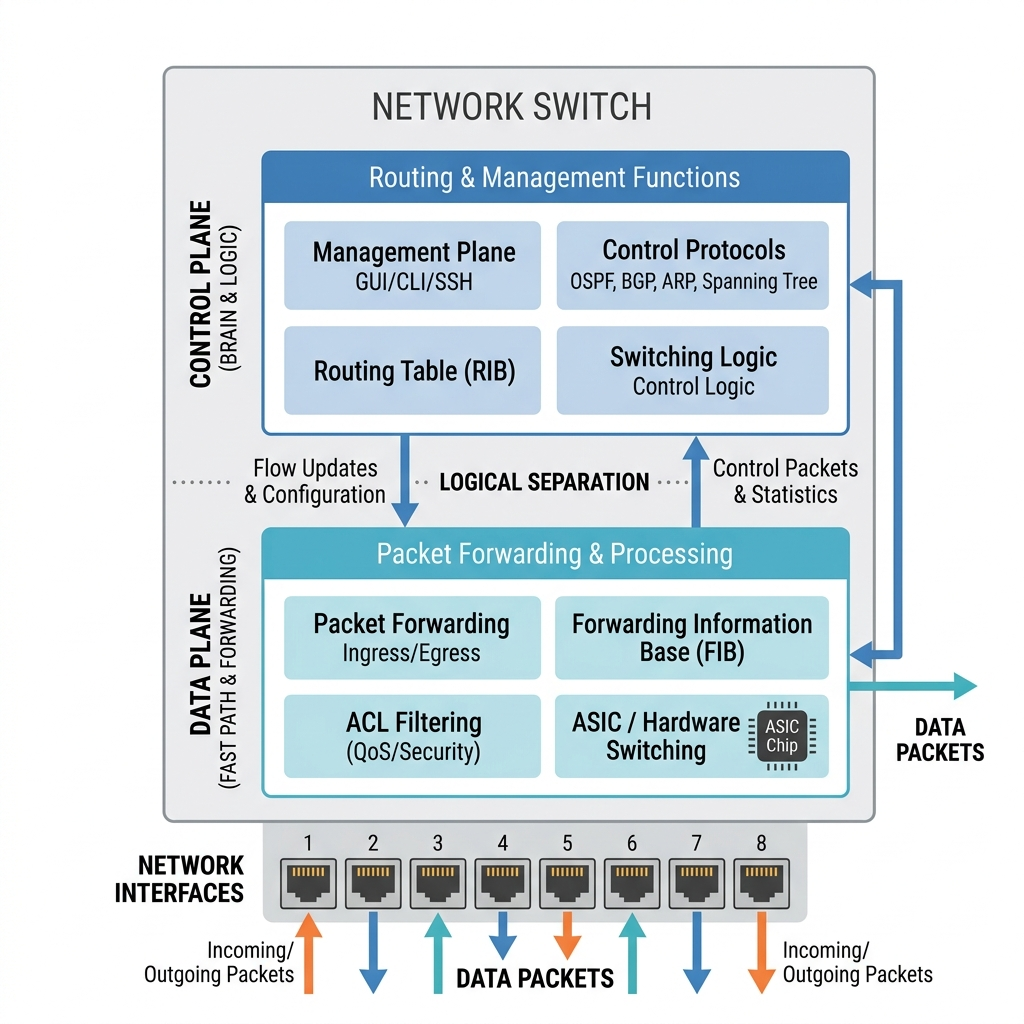
\includegraphics[width=0.7\textwidth]{images/network_planes.png}
    \caption{Logical architecture: separation between Control Plane and Data Plane in a network device.}
\end{figure}
In the past, the dominant network architecture was based on huge proprietary \textit{modular chassis} (e.g. large Cisco core switches), expensive and difficult to scale gradually. The modern switch, driven by the hyperscale needs of the cloud, has abandoned chassis in favor of the \textbf{Fixed Form Factor} (1U or 2U), often called \textit{White-box switch}.

\subsection{Software-Defined Networking (SDN) and SONiC}
\begin{figure}[H]
    \centering
    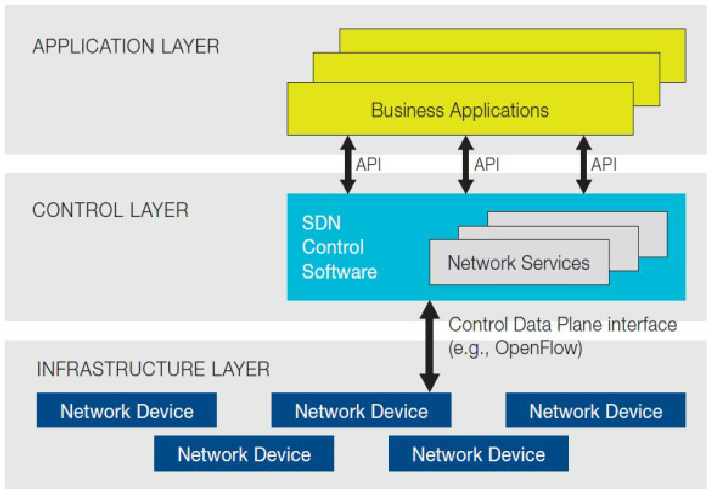
\includegraphics[width=0.7\textwidth]{images/sdn.png}
    \caption{SDN Model: network intelligence is abstracted from the underlying physical infrastructure.}
\end{figure}
The great revolution was the conceptual separation into two planes:
\begin{figure}[H]
    \centering
    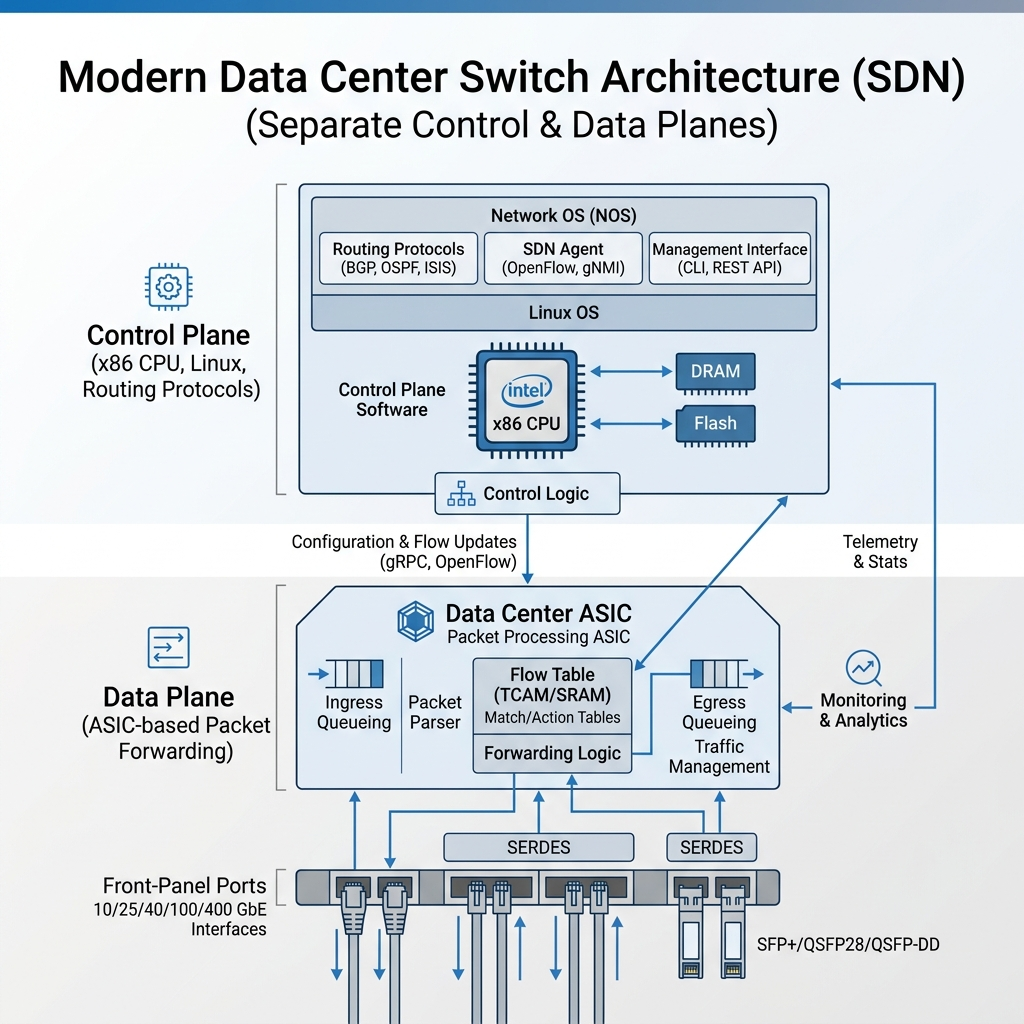
\includegraphics[width=0.8\textwidth]{images/sdn_control_plane.png}
    \caption{Architectural detail of the separation between ASIC (Data Plane) and x86 CPU (Control Plane).}
\end{figure}
\begin{enumerate}
    \item \textbf{Data Plane:} dedicated hardware (often commodity ASICs, e.g., Broadcom chips) that \textit{forwards} packets in a non-blocking way at \textit{line-rate} speed. The introduction of a frame into this hardware ASIC adds a negligible latency of about \textbf{600 ns}.
    \item \textbf{Control Plane:} an actual PC (often based on \textbf{Intel Celeron} or similar processors) integrated into the chassis, which manages network logic (BGP, OSPF). Being a full Linux PC, software can be compiled on it (e.g. running the VSCode editor directly inside the switch to edit scripts).
\end{enumerate}

\begin{warningbox}[Running vs Startup Config]
In network operating systems, managing the Control Plane memory is vital. Parameter modifications (e.g. via CLI) occur in the \textbf{Running Configuration} (located in volatile RAM); they take effect immediately but disappear in the event of a shutdown or blackout. To make them permanent, they must be saved to the \textbf{Startup Configuration} (flash memory/NVRAM) using the \texttt{write} (or \texttt{copy running-config startup-config}) command. Many catastrophic outages (impossible to debug later) arise from sudden reboots of devices whose configurations were never persisted to disk.
\end{warningbox}
\begin{figure}[H]
    \centering
    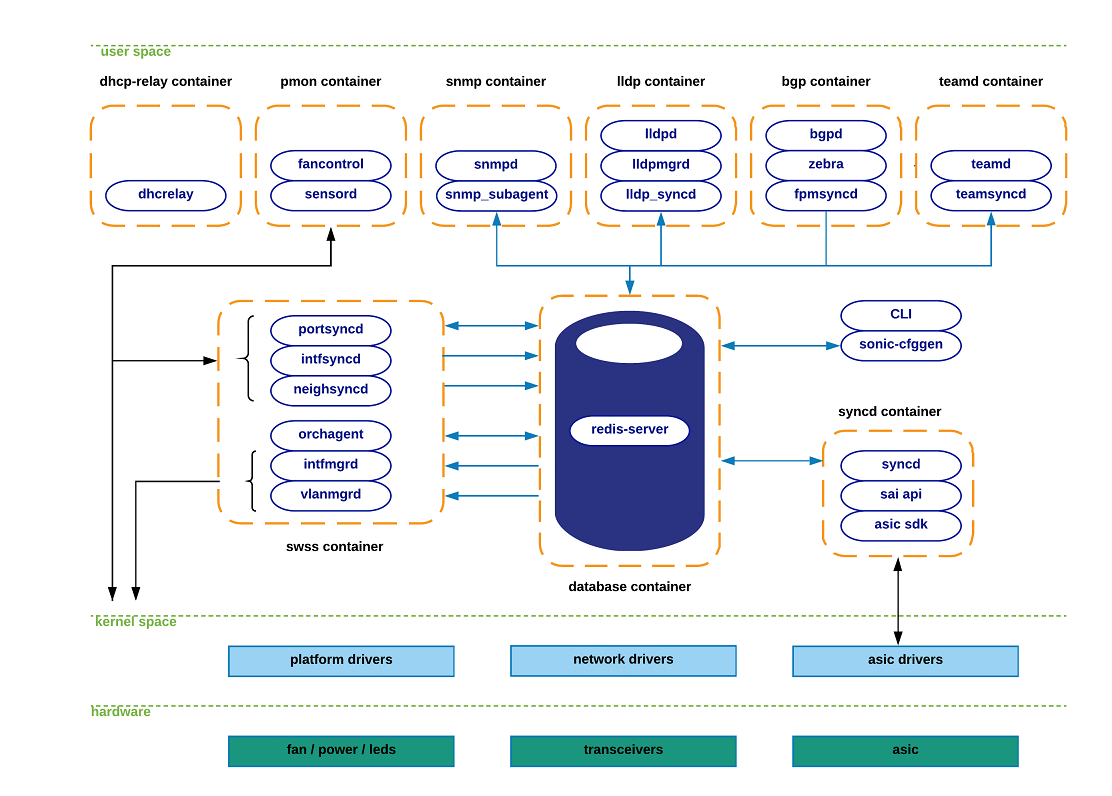
\includegraphics[width=0.7\textwidth]{images/sonic.png}
    \caption{SONiC Architecture: each network function runs in its own Docker container communicating via Redis.}
\end{figure}
Hardware-software disaggregation led to the birth of open-source Network Operating Systems (NOS) like \textbf{SONiC} (Software for Open Networking in the Cloud, created by Microsoft). Booted via the ONIE bootloader, SONiC treats the switch like a standard server, running each routing daemon inside isolated \textit{Docker containers}.

\subsubsection{The OpenFlow API and the Firewall Sandwich}
To instruct the Data Plane on how to forward packets, the Control Plane (or a centralized controller) uses communication protocols, the most famous of which is the \textbf{OpenFlow API}. This allows programmatic manipulation of the \textit{Flow Tables} inside the ASIC.
Thanks to this abstraction, architectures like the \textbf{Firewall Sandwich} are created: the SDN controller (OpenFlow) instructs the switch to divert all incoming traffic to a series of hardware firewalls placed in parallel (the "filling" of the sandwich). Once inspected, the traffic returns to the switch which routes it to its final destination, load-balancing and ensuring linear scalability of security, transparently.

\begin{figure}[H]
    \centering
    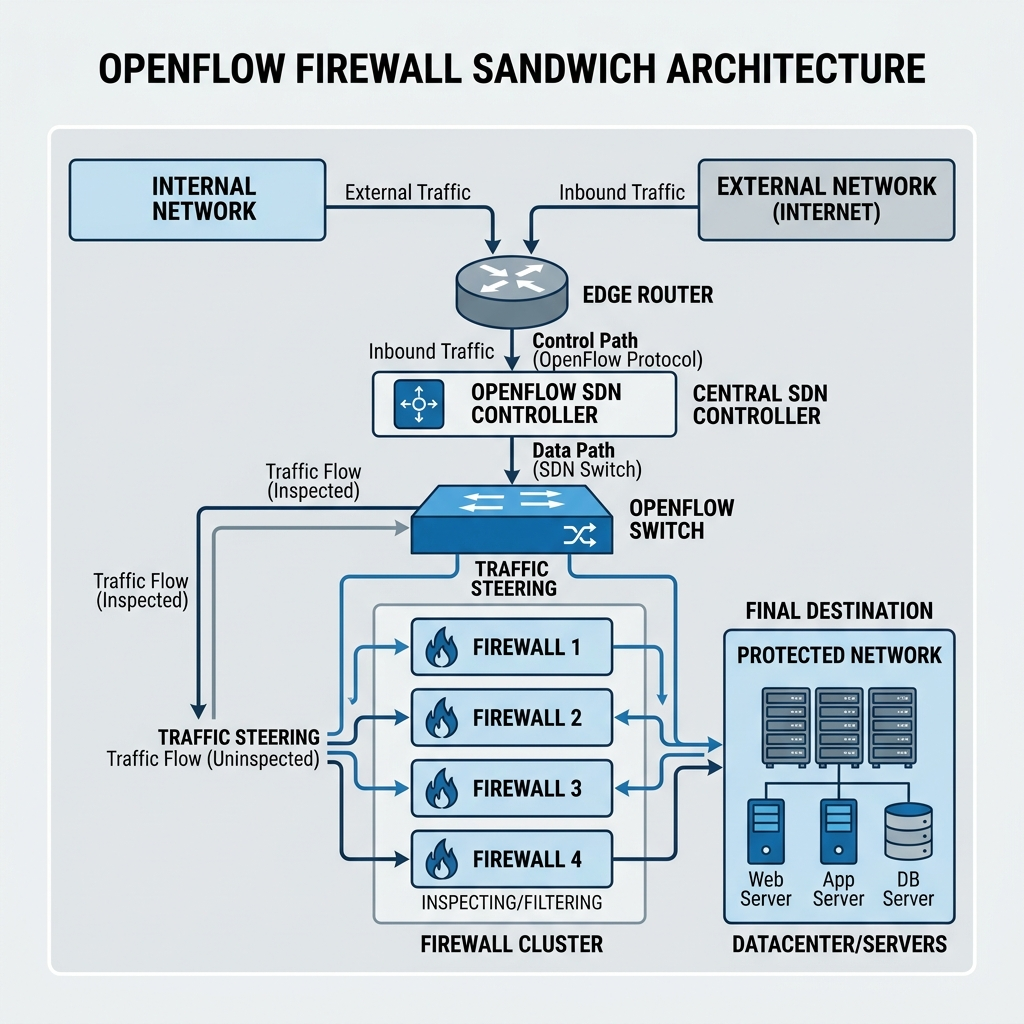
\includegraphics[width=0.7\textwidth]{images/openflow_sandwich.png}
    \caption{Firewall Sandwich architecture governed via SDN and OpenFlow.}
\end{figure}

\section{Network Topologies: From 3-Tier to Spine-and-Leaf}
Historically, datacenters adopted a \textbf{3-tier} topology (Access, Distribution, Core), optimized for \textbf{North-South} (client-server) traffic. 
Redundant links inevitably created physical loops. If a broadcast packet started to cycle, it triggered a catastrophic \textbf{Broadcast Storm} capable of paralyzing the entire datacenter in seconds. To prevent this, the \textbf{STP (Spanning Tree Protocol)} was used, which preemptively disabled redundant physical links. The flaws of STP were multiple: huge bandwidth waste (up to 50\% of the laid cables remained dormant) and slow convergence times in case of failure (topology recalculations momentarily blocked traffic).

Today, the explosion of microservices, cloud, and AI has made \textbf{East-West} (server-to-server) traffic absolutely dominant. The standard topology of modern data centers has become \textbf{Spine-and-Leaf} (derived from \textit{Clos} networks):

\begin{figure}[H]
    \centering
    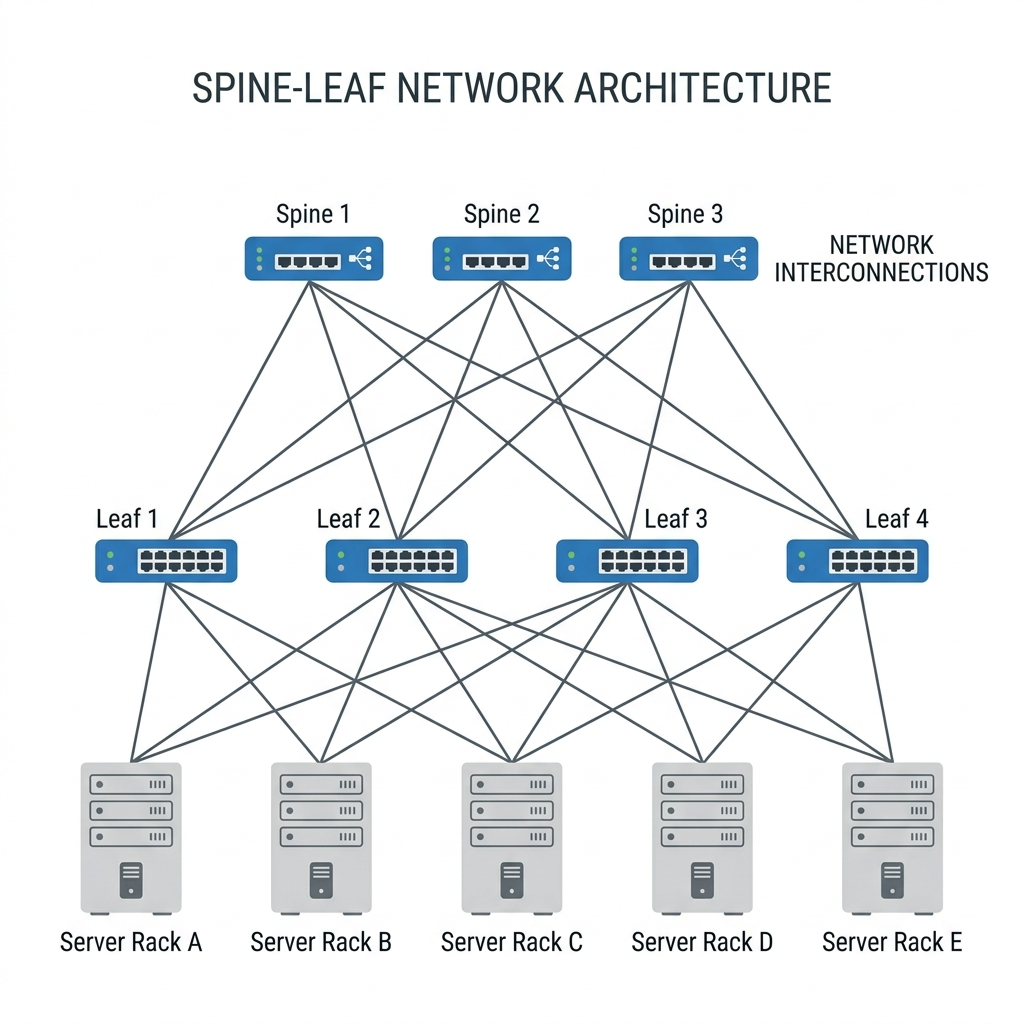
\includegraphics[width=0.8\textwidth]{images/spine_leaf_arch.png}
    \caption{Spine-Leaf Architecture: Full-Mesh connection between Leaf layer and Spine layer.}
\end{figure}

The architecture is developed on two rigorous physical layers:
\begin{itemize}
    \item \textbf{Leaf Layer (Access):} Consists of ToR (Top-of-Rack) switches. Physical servers connect \textit{only} to these switches. In turn, Leaf switches \textbf{are never connected to each other}.
    \item \textbf{Spine Layer (Backbone):} The central aggregation layer. Every single Leaf switch has at least one fiber uplink to \textbf{every} single Spine switch (creating a \textit{Full-Mesh} configuration between the two layers). Spine switches also \textbf{never talk directly to each other}.
\end{itemize}

\begin{tipbox}[Advantages and Oversubscription]
\begin{itemize}
    \item \textbf{Deterministic Latency:} Every server communicates with any other server taking exactly the same number of hops (1 logical hop: \textit{leaf $\rightarrow$ spine $\rightarrow$ leaf}).
    \item \textbf{ECMP (Equal-Cost Multi-Path):} Without traditional physical loops, STP is replaced by L3 routing. Traffic is uniformly load-balanced across \textit{all} available uplinks. If a Spine switch fails, the network degrades only fractionally in bandwidth, but does not go down.
    \item \textbf{Oversubscription Ratio:} The ratio between total downlink bandwidth (towards servers) and uplink bandwidth (towards Spines). A typical cloud uses 3:1 ratios. HPC or AI environments demand a \textbf{1:1} ratio (called \textit{Non-blocking}), ensuring all servers can transmit at maximum concurrently without bottlenecks.
\end{itemize}
\end{tipbox}

\section{Network Segmentation and Virtualization}

\subsection{Jumbo Frames and MTU}
Before logically fragmenting the network, it is essential to define its maximum payload. The standard \textbf{MTU (Maximum Transmission Unit)} in Ethernet is 1500 bytes. However, in datacenter environments (especially for storage traffic), segmenting huge files into 1.5 KB blocks causes unsustainable CPU overhead to process millions of headers. \textbf{Jumbo Frames} are therefore enabled, raising the MTU to \textbf{9000 bytes (9 KB)}.
The operational trap is fragmentation: the MTU must be configured strictly identical on every single switch and server along the path, otherwise performance will drop drastically or packets will be silently lost (\textit{black holing}).

\subsection{VLAN (Virtual LAN)}
The classic Ethernet header contains a destination MAC address (6 bytes), a source MAC (6 bytes) and an EtherType field (2 bytes). VLANs (IEEE 802.1Q standard) allow a physical network to be divided into multiple logical broadcast domains by inserting a 4-byte tag right after the source MAC. 
This 802.1Q tag includes a TPID field (indicating the presence of the VLAN) and a TCI, which in turn contains 3 bits for priority (QoS) and \textbf{12 bits for the VLAN identifier (VID)}. Since the VLAN ID is exactly 12 bits long, the unbreakable theoretical limit is \textbf{4094 usable networks} ($2^{12}-2$), an absolutely insufficient number for modern multi-tenant cloud providers that must host hundreds of thousands of isolated networks.

\subsection{VXLAN and Overlay}
To overcome the architectural rigidity and the 4096-network limit of traditional VLANs, the modern cloud datacenter uses \textbf{VXLAN (Virtual eXtensible LAN)}. It is an \textit{overlay} protocol (Mac-in-UDP) that encapsulates entire Layer 2 (Ethernet) packets within Layer 3 transport packets (UDP/IP). 
This raises the limit to \textbf{16 million isolated virtual networks} (thanks to a 24-bit VNI identifier) and allows the creation of arbitrary Layer 2 broadcast domains over a Layer 3 physical routing infrastructure. This means that two virtual machines can believe they are connected to the same physical switch (same L2 subnet), even if they are located in two physically distant L3-routed racks.

\section{High-Performance Fabric (HPC and AI)}
In HPC and AI training contexts, software overhead becomes the primary enemy. As seen, a frame crosses the switch hardware (the cut-through ASIC) in about \textbf{600 ns}. However, just to pass the data through the TCP/IP protocol software stack inside the server's operating system (interrupt handling, buffer allocation), about \textbf{70 $\mu$s} of latency are introduced (over 100 times the switching time), a value that TCP inventor Vint Cerf associated with the problem of \textit{bufferbloat} (the destructive accumulation of packets in intermediate buffers).

In these scenarios, \textbf{InfiniBand} dominates, a network that offers latencies of 1-3 $\mu$s. The secret is the implementation of the \textbf{RDMA (Remote Direct Memory Access)} protocol, which allows a server to write directly into the RAM memory of another server, completely bypassing the intervention of the CPU and the receiving operating system.
Today, RDMA is also available on advanced Ethernet networks via the \textbf{RoCE} (RDMA over Converged Ethernet) protocol.

\begin{definitionbox}[Full Fat Tree]
To avoid \textit{overbooking} (uplink overload) critical for HPC, the \textbf{Full Fat Tree} topology is used: a non-blocking structure where the bandwidth towards the upper layers is exactly equal to that of the lower layers, ensuring bottleneck-free communications.
\end{definitionbox}
